\documentclass{article}

\usepackage[a4paper,left=1in,right=1in,top=1in,bottom=1in,footskip=.25in]{geometry}
\usepackage{listings}
\usepackage{lipsum}
\usepackage{graphicx}
\usepackage{afterpage}
\usepackage{xcolor}
\usepackage{fancyhdr}
\usepackage{float}
\usepackage{helvet}
\usepackage{url}
\usepackage[toc,page]{appendix}
\usepackage[final]{pdfpages}
\usepackage[hidelinks]{hyperref}

\renewcommand{\familydefault}{\sfdefault}

\pagestyle{fancy}

\graphicspath{{./IMAGES/}}

\lstset{
	escapeinside={/*@}{@*/},
	language=Java,	
	basicstyle=\ttfamily\fontsize{8.5}{12},
	numbers=left,
	numbersep=2pt,    
	xleftmargin=2pt,
	frame=tb,
	columns=fullflexible,
	showstringspaces=false,
	tabsize=4,
	keepspaces=true,
	showtabs=false,
	showspaces=false,
	morekeywords={inline,public,class,private,protected,struct},
	captionpos=b,
	lineskip=-0.4em,
	aboveskip=10pt,
	extendedchars=true,
	breaklines=true,
	prebreak = \raisebox{0ex}[0ex][0ex]{\ensuremath{\hookleftarrow}},
	keywordstyle=\color[rgb]{0,0,1},
	commentstyle=\color[rgb]{0.133,0.545,0.133},
	stringstyle=\color[rgb]{0.627,0.126,0.941},
}

\title{USB/Bluetooth Media Controller\\Final Report}
\author{40056761\\SET09118\\Edinburgh Napier University}
\date{22-04-2016}
\makeatletter
\lhead{SET09118: Final Report}
\rhead{40056761}


\begin{document}
		
	\maketitle
	
	\section*{Abstract}	
		This document is the final report and a summary to the "USB/Bluetooth Media Controller" project started in February [Appendix \ref{IPP}] [Appendix \ref{Interim}]. The goal of the project was to research, develop and evaluate a micro-controller based system and mobile application.		
				
	\newpage
		
	\pagenumbering{arabic}
		
	\tableofcontents
	
	\listoffigures
	
	\listoftables
	
	\lstlistoflistings
		
	\newpage
		
	\section{Introduction}
		\subsection{Background and Rational}
			The goal for this project was to produce a system that would allow users to interact with their PC media in a more intuitive manner. From tape cassettes to compact discs and finally to digital MP3 files, the way in which media is stored and experienced had changed dramatically over the last twenty years but the way that user interact with their media has remained stagnant.
			
			While playing or pausing media, changing track or altering volume are typically not difficult tasks for users, it can often be complicated when other applications are in use. Many companies have attempted to solve this issue by incorporating media control keys into keyboards, however these buttons are often in hard to reach locations or only work with specific applications.
			
			For the reasons mentioned above, it is clear that a independent media-controller, that supports a multitude of media application would be a popular device for many PC fanatics. One of the key deliverables of this project is the aforementioned media controller, the other is a companion mobile application to control the device remotely.
					
		\subsection{Aims and Deliverables}
			As stated previously, the two major deliverables discussed in this report are; a micro-controller based media controller and an Android mobile application to control said device. The aim of both deliverables is to simplify the way a user interacts with media, and this was a major consideration for design and implementation of the systems.
			
			In an ideal world, a media controller would be able interface with any device, and any media application, allowing for complete control without the need for installation and configuration. Unfortunately, the real world is not as fair, and limitations must be imposed to keep implementation time reasonable.
			\begin{itemize}
				\item Function on a PC with a Windows operating system
				\item Media application support for Google Play Music
			\end{itemize}			
			
			

%			constraint = external
%			limitation = self imposed 

	
	\section{Design}
		\subsection{Physical System Design}
			\lipsum[1]
			
			\begin{table}[h]
				\centering
				\caption{A usage table of the HID commands utilized by the media-controller}
				\label{my-label}
				\begin{tabular}{|r|r|r|}
					\hline
					\multicolumn{1}{|l|}{Usage ID} & \multicolumn{1}{l|}{Usage Name} & \multicolumn{1}{l|}{Usage Type} \\ \hline
					0xCD                           & Play/Pause                      & OSC                             \\
					0xB0                           & Play                            & OOC                             \\
					0xB1                           & Pause                           & OOC                             \\
					0xB3                           & Fast Forward                    & OOC                             \\
					0xB4                           & Rewind                          & OOC                             \\
					0xB5                           & Scan Next Track                 & OSC                             \\
					0xB6                           & Scan Previous Track             & OSC                             \\
					0xB7                           & Stop                            & OSC                             \\
					0xE2                           & Mute                            & OOC                             \\
					0xE9                           & Volume Increment                & RTC                             \\
					0xEA                           & Volume Decrement                & RTC                             \\ \hline
				\end{tabular}
			\end{table}
		
		\subsection{Mobile Application Design}
			\lipsum[1]

	\section{Implementation}
		\subsection{Micro-controller Implementation}
			\lipsum[1]
			
		\subsection{Mobile Application Implementation}
			\lipsum[1]
			
	\section{Results}
		\subsection{Achievements}
			\lipsum[1]
			
		\subsection{Recommendations}
			\lipsum[1]
			
	\section{Future Work}
		\lipsum[1]
	
	\section{Conclusion}
		\lipsum[1]
		
	\section{Evaluation of Achievement}
		\lipsum[1]
		
	\bibliographystyle{ieeetran}
	
	\bibliography{final}

	\newpage

	\begin{appendices}

		\section{Arduino Media-Controller Source Code}
			\lstinputlisting[caption = mediaController\_debounce.ino, nolol]{../../ARDUINO/mediaController_debounce/mediaController_debounce.ino}
			\newpage
			
		\section{Arduino Media Key Library}
			\lstinputlisting[title = Media.h, nolol]{../../ARDUINO/Media/Media.h}
			\newpage
			\lstinputlisting[title = Media.cpp, nolol]{../../ARDUINO/Media/Media.cpp}
			\newpage
			
		\section{Android Application Source code}
			\lstinputlisting[title = MainActivity.java, nolol]{../../ANDROID/MediaController/app/src/main/java/uk/co/sam/mediacontroller/MainActivity.java}
			\newpage
			
			\lstinputlisting[title = BluetoothHandler.java, nolol]{../../ANDROID/MediaController/app/src/main/java/uk/co/sam/mediacontroller/BluetoothHandler.java}
			\newpage
					
		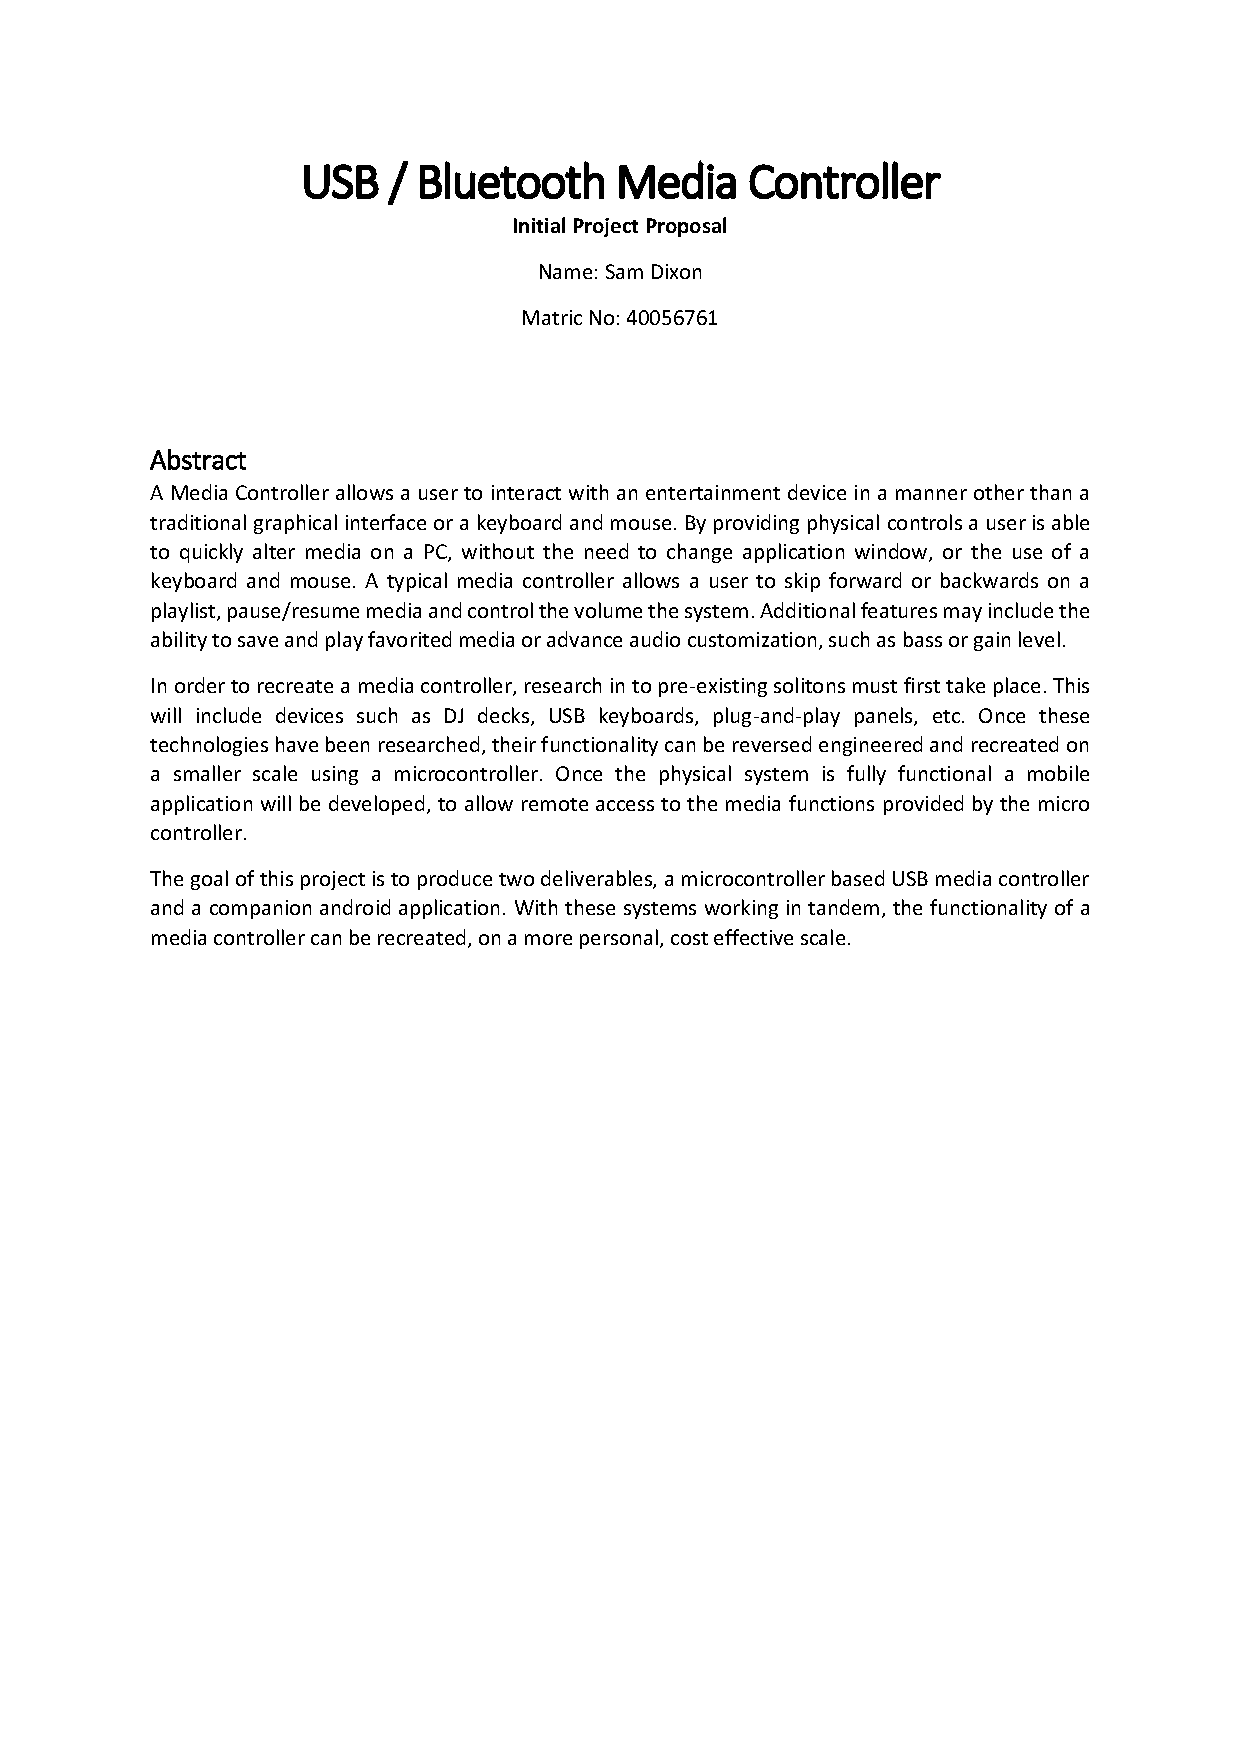
\includepdf[scale = 0.8, pages=1,pagecommand=\section{Initial Project Proposal}\label{IPP}]{../IPP/SET09118_IPP.pdf}
		\includepdf[scale = 0.8, pages=2-,pagecommand={}]{../IPP/SET09118_IPP.pdf}
		\newpage
	
		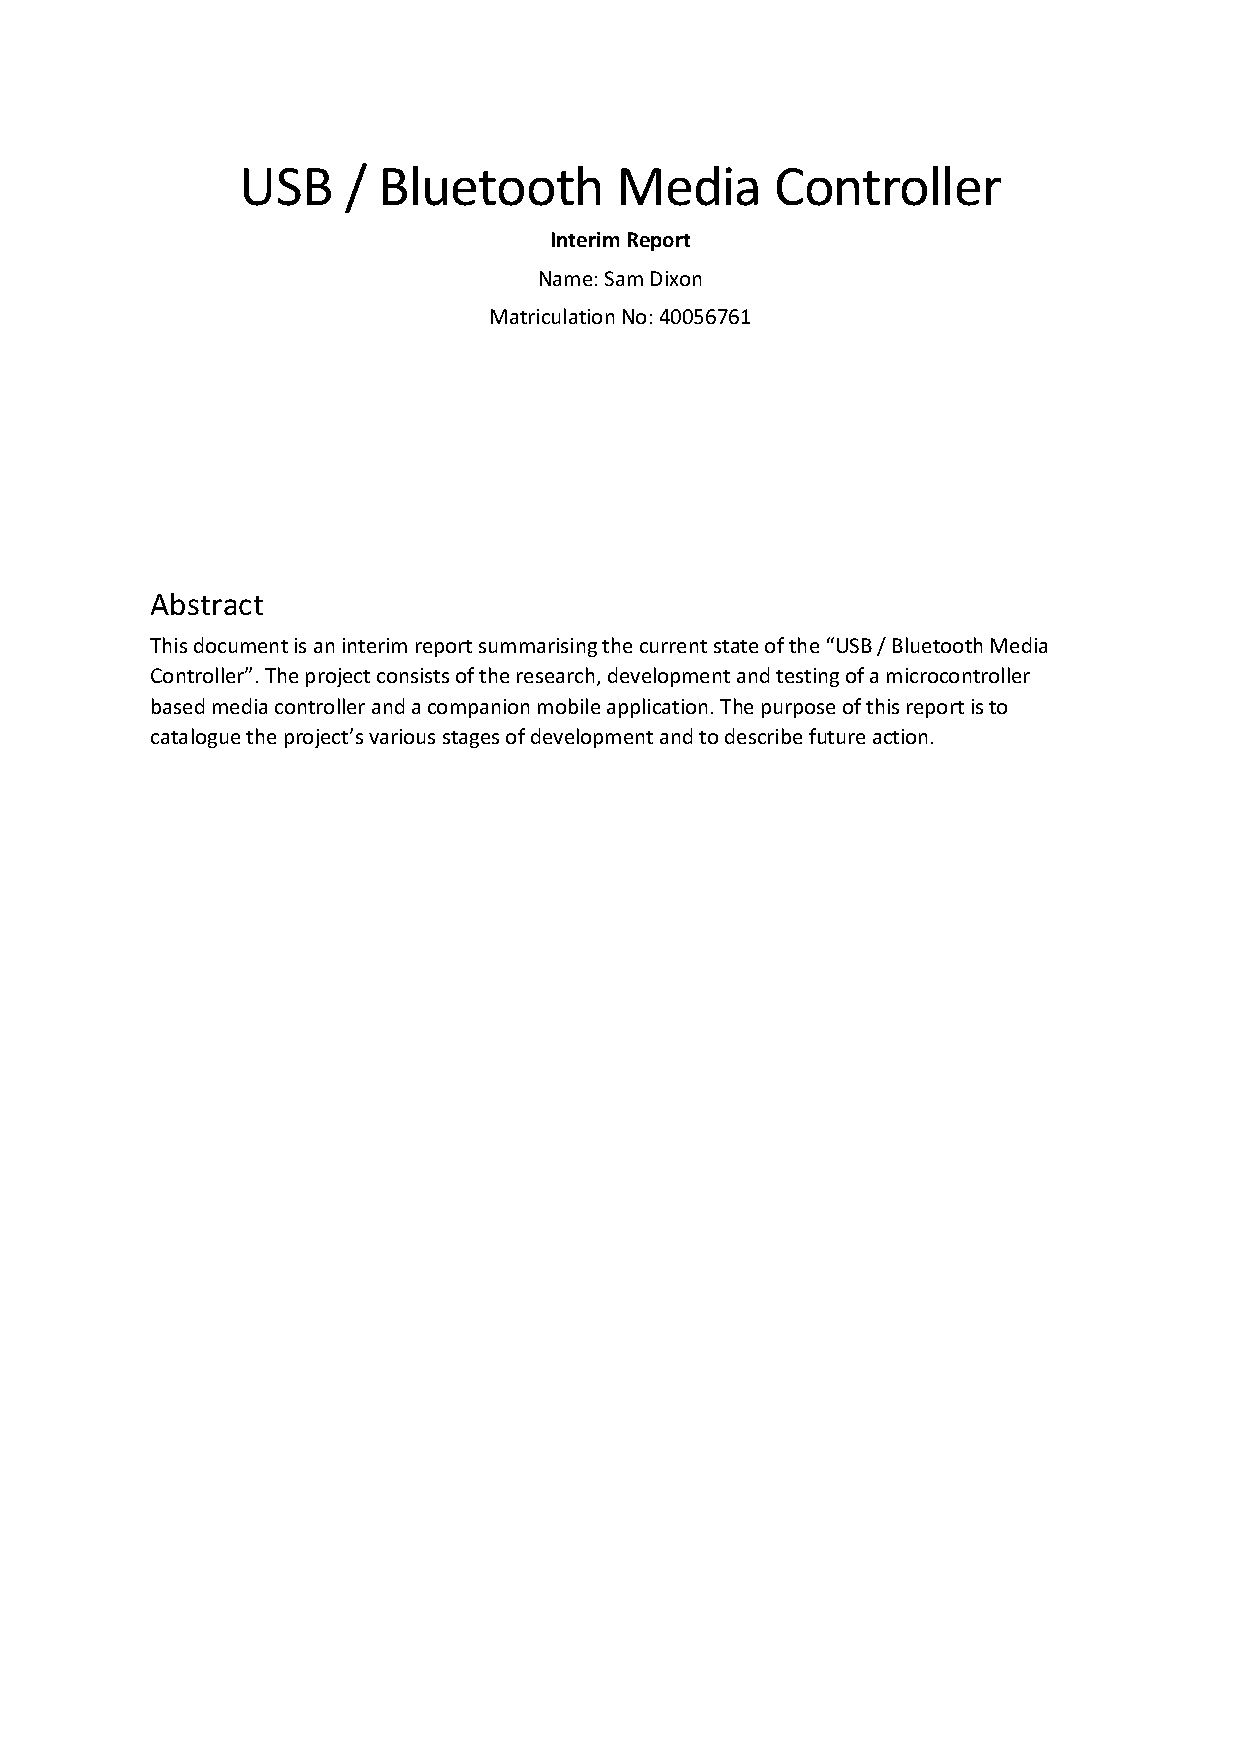
\includepdf[scale = 0.8, pages=1,pagecommand=\section{Interim Report}\label{Interim}]{../INTERIM/SET09118_INTERIM.pdf}
		\includepdf[scale = 0.8, pages=2-,pagecommand={}]{../INTERIM/SET09118_INTERIM.pdf}
		\newpage	

		 		
	\end{appendices}

\end{document}